\begin{landscape}
\begin{figure}[!]
    \centering
    \captionlistentry{Level Scheme of $^{154}$Gd. The gate on the $6_{gs}^+\rightarrow 4_{gs}^+$ transition (346 keV) $\gamma$-component in the ground state. The lines shown are in coincidence. The levels are organized by band. The lower levels of the band, unseen by gamma rays in this gate, are in blue.}
    \label{fig:154_6to4}
    \begin{subfigure}{1.4\textwidth}
    \caption*{\centering \fontsize{10pt}{12pt}Figure \ref{fig:154_6to4}. Level Scheme of $^{154}$Gd. The gate on the $6_{gs}^+\rightarrow 4_{gs}^+$ transition (346 keV) $\gamma$-component in the ground state. The lines shown are in coincidence. The levels are organized by band. The lower levels of the band, unseen by gamma rays in this gate, are in blue.}
    \end{subfigure}
\end{figure}
\clearpage
\begin{figure}
    \ContinuedFloat
    \begin{subfigure}{1.4\textwidth}
    \includegraphics[scale=0.33]{154GdTablesAndFigs/154Gd_6to4.eps}
    \label{fig:154_6to4level}
    \end{subfigure}
\end{figure}
\end{landscape}
\begin{figure}
    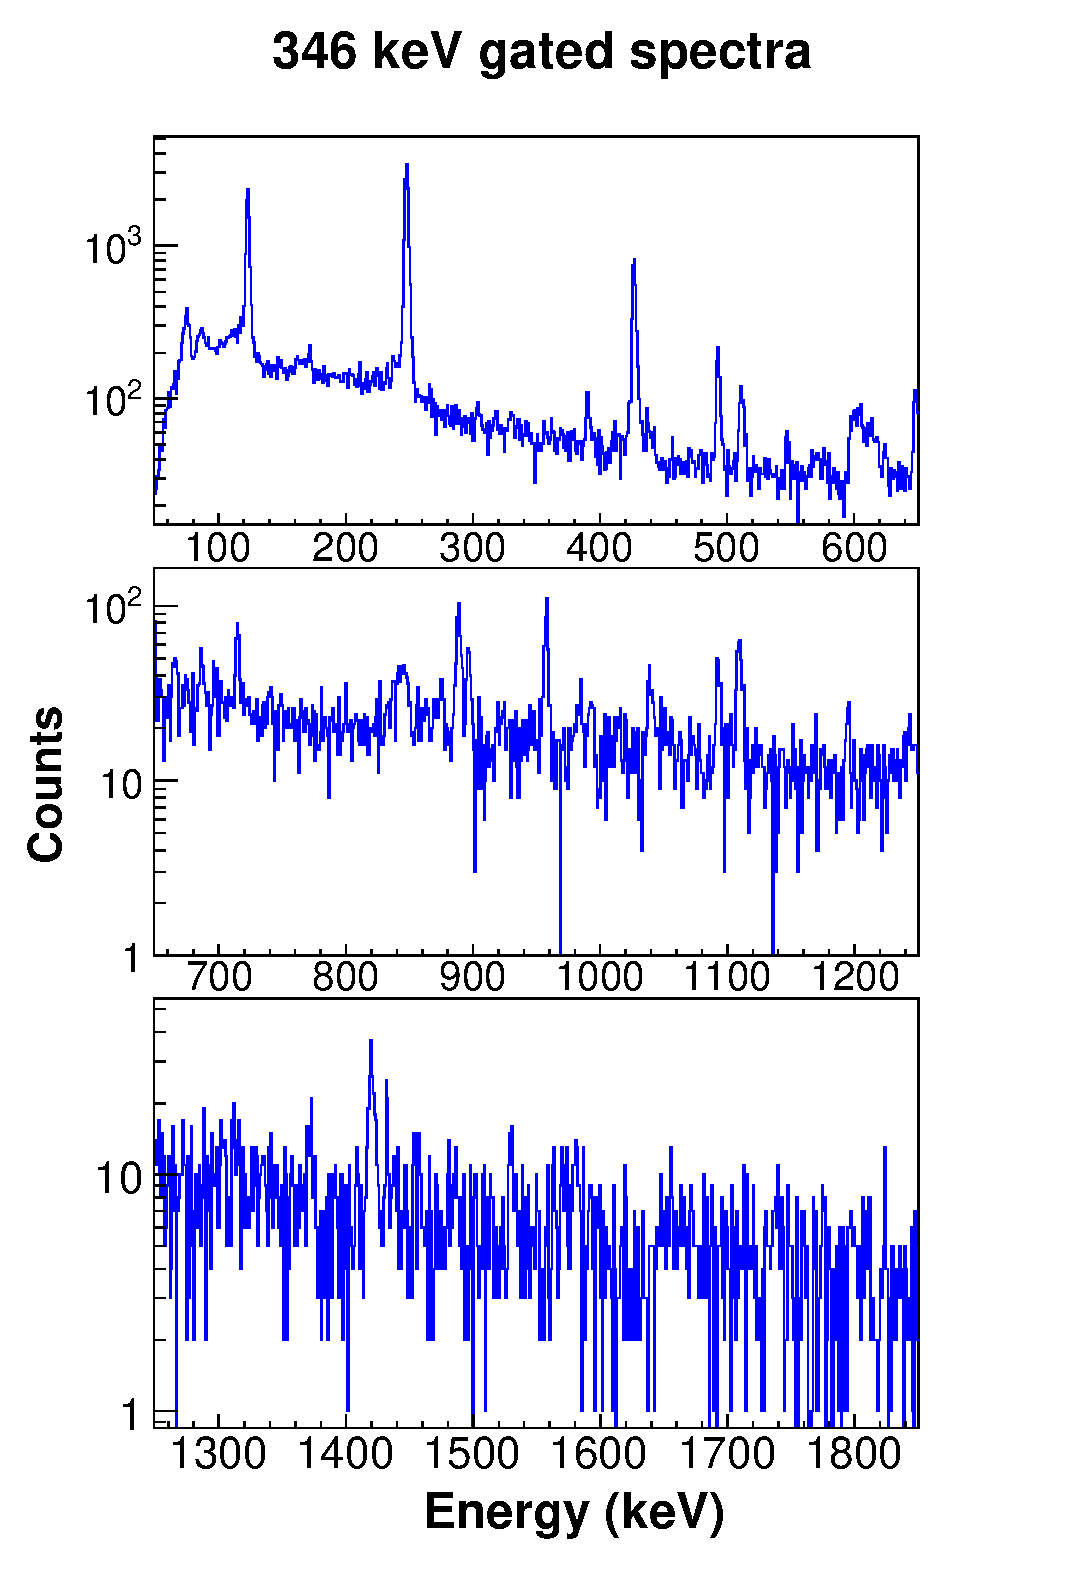
\includegraphics[scale=1.3]{154GdTablesAndFigs/346_gamma.eps}
    \caption{Gamma spectrum gated on 346 keV, corresponding to the $6_{gs}^+\rightarrow 4_{gs}^+$ transition. Several transitions have been labeled, corresponding to the level scheme in Figure \ref{fig:154_6to4}.}
    \label{fig:154_6to4spec}
\end{figure}